\documentclass{article}
\usepackage[utf8]{inputenc}
\usepackage{multicol}
\usepackage{calc}
\usepackage{ifthen}
\usepackage[portrait]{geometry}
\usepackage{amsmath,amsthm,amsfonts,amssymb}
\usepackage{color,graphicx,overpic}
\usepackage{hyperref}
\usepackage{tabularx}
\usepackage{graphicx}

\graphicspath{ {images/} }

\newenvironment{nosepitemize}
{ \begin{itemize}
    \setlength{\itemsep}{0pt}
    \setlength{\parskip}{0pt}
    \setlength{\parsep}{0pt}     }
{ \end{itemize}                  }

\newenvironment{nosepenumerate}
{ \begin{enumerate}
    \setlength{\itemsep}{0pt}
    \setlength{\parskip}{0pt}
    \setlength{\parsep}{0pt}     }
{ \end{enumerate}                  }

% Turn off header and footer
\pagestyle{empty}

% Don't print section numbers
\setcounter{secnumdepth}{0}

% This sets page margins to .5 inch if using letter paper, and to 1cm
% if using A4 paper. (This probably isn't strictly necessary.)
% If using another size paper, use default 1cm margins.
\ifthenelse{\lengthtest { \paperwidth = 11in}}
    { \geometry{top=.5in,left=.5in,right=.5in,bottom=.5in} }
    {\ifthenelse{ \lengthtest{ \paperwidth = 297mm}}
        {\geometry{top=1cm,left=1cm,right=1cm,bottom=1cm} }
        {\geometry{top=1cm,left=1cm,right=1cm,bottom=1cm} }
    }

\begin{document}

\begin{center}
     \section{Facilitating Dialogue Cheat Sheet}
\end{center}

\begin{multicols}{2}

\noindent
\textbf{Dialogue} and \textbf{Healthy Conflict} are essential skills for high performing teams and organizations to master.

\begin{nosepitemize}
    \item \textbf{To improve decision making}, by hearing perspectives and exploring our options thoroughly.
    \item \textbf{To generate commitment}. We don't need consensus, but we do need to give everyone a chance to have their voices heard.
    \item \textbf{To move faster}. By exploring options carefully, we will create greater alignment, greater commitment, improve our understanding of risks, and find a better path forwards once we start to implement.
    \item \textbf{To build psychological safety}. Leaders should create space to surface disagreement in a safe and constructive way in order to build a \textit{generative} culture.
\end{nosepitemize}

\end{multicols}

\begin{center}
\section{Kantor's 4-Player Model}
\end{center}

\begin{multicols}{2}

\noindent
Kantor's model posits that there are 4 possible speech 'acts'.

Communication problems occur when individuals become 'stuck' over-using one of these acts, or when certain sequences become entrenched, undermining group learning and decision making.

\centerline{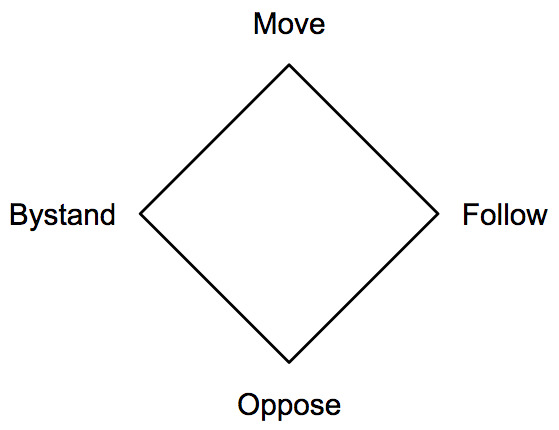
\includegraphics[width=0.6\linewidth]{4-player-model.png}}

\begin{nosepenumerate}
    \item The \textbf{Move} act establishes direction and sets the team in motion.
    \item The \textbf{Follow} act provides support for the move and serves as the function of completion.
    \item The \textbf{Oppose} act questions the move that has been initiated.
    \item The \textbf{Bystand} act provides perspective and invites the team to reflect.
\end{nosepenumerate}

\subsection{Why we need these acts}

\begin{nosepitemize}
    \item Without a mover, the team lacks direction.
    \item Without those who will follow, work won’t get completed.
    \item Without an opposer, legitimate concerns are ignored.
    \item Without bystanders, we lose perspective and fail to explore all angles.
\end{nosepitemize}

\subsection{In practice}

You should:

\begin{nosepitemize}
    \item Be aware of your own tendencies.
    \item Strike a balance.
    \item Cite the acts (e.g. \textit{“I am going to play the Oppose role”}; \textit{“I am going to act as Bystander”}; etc.)
\end{nosepitemize}

\noindent
Facilitators should:

\begin{nosepitemize}
    \item Listen to the balance of the room.
    \item Reflect back to the room the acts they're seeing and hearing.
    \item Encourage participants to play different roles, especially to get discussion “unstuck”.
    \item Remind participants to state the acts they're performing.
\end{nosepitemize}

\end{multicols}

\begin{center}
\section{Bohmian Dialogue}
\end{center}

\begin{multicols}{2}

\noindent
Bohm distinguishes between \textit{discussion} and \textit{dialogue}.

\textbf{Discussion} is like a game, with winners and losers: one sets out to prove one's point, or to get commitment to one's ideas.

The intent of \textbf{Dialogue} is not to win, but simply to understand something about how the group is thinking by surfacing assumptions and cognitive errors. If a mistake is discovered, everyone wins.

To engage in dialogue, one should surface one's \textbf{basic assumptions}, i.e. the assumptions, prejudices and defensive routines  that are typically automatically invoked without our awareness.

\section{How does this help?}

As Peter Senge notes: \textit{“Through dialogue, we become observers of our own thinking.”} We can \textit{“begin to take a more creative, less reactive stance toward thought.”}

\section{In Practice}

You should:

\begin{nosepitemize}
    \item Maintain awareness of your internal feelings and responses.
    \item “Suspend your assumptions”: surface them so that you and others can learn about how you are thinking.
    \item Focus on learning about how others are thinking, rather than being right or winning points.
\end{nosepitemize}

\noindent
Facilitators should:

\begin{nosepitemize}
    \item Ask participants to regard one another as colleagues “in mutual quest for deeper insight and clarity”.
    \item Encourage participants to “suspend” their assumptions by making them visible to the group.
    \item “Hold the Context” of dialogue: if the group turns to point-seeking discussion, bring the group back to dialogue.
\end{nosepitemize}

\end{multicols}

\end{document}